\begin{figure}[ht]
\centering
\begin{minipage}{.5\textwidth}
\centering
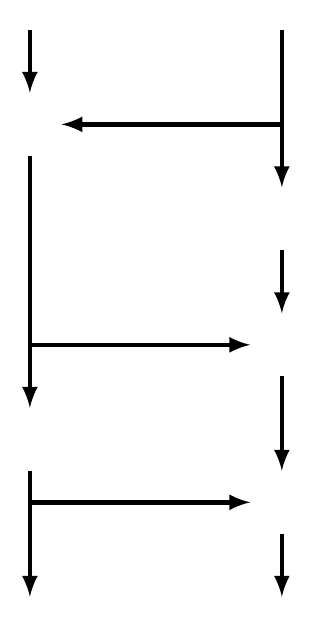
\begin{tikzpicture}[scale=0.8,ultra thick,>=latex]
% Reference grid (temporary)
%\draw[help lines] (0,0) grid (16,16);

% Inputs A and B
\drawMixerInputs
\draw[->] (1,15) to (1,14);
\draw[->] (5,15) to (5,12.5);

% Left adder 
\drawAdder{0.5}{14}
\draw[->] (5,13.5) to (1.5,13.5);

% Rotation
\drawRot{5}{12}

% Right adder
\drawAdder{4.5}{10.5}
\draw[->] (5,11.5) to (5,10.5);
\draw[->] (1,10) to (4.5,10);

% Rotation
\drawRot{1}{8.5}
\draw[->] (1,13) to (1,9);

% XOR
\drawXOR{5}{7.5}
\draw[->] (1,7.5) to (4.5,7.5);
\draw[->] (5,9.5) to (5,8);

% Outputs A' and B'
\draw[->] (1,8) to (1,6);
\draw[->] (5,7) to (5,6);
\drawMixerOutputs{10}
\end{tikzpicture}
\end{minipage}%
%
%
\begin{minipage}{.5\textwidth}
\centering
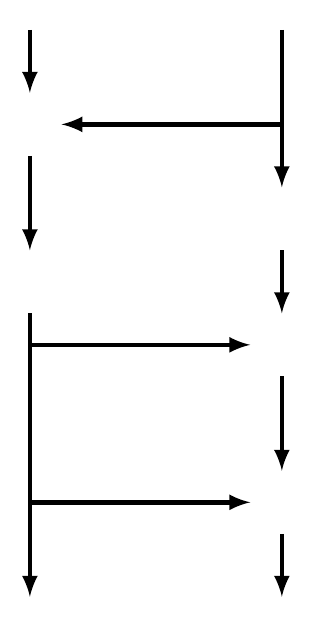
\begin{tikzpicture}[scale=0.8,ultra thick,>=latex]
% Reference grid (temporary)
%\draw[help lines] (0,0) grid (16,16);

% Inputs A and B
\drawMixerInputs
\draw[->] (1,15) to (1,14);
\draw[->] (5,15) to (5,12.5);

% Left adder 
\drawAdder{0.5}{14}
\draw[->] (5,13.5) to (1.5,13.5);

% Rotation
\drawRot{5}{12}

% Rotation
\drawRot{1}{11}
\draw[->] (1,13) to (1,11.5);

% Right adder
\drawAdder{4.5}{10.5}
\draw[->] (5,11.5) to (5,10.5);
\draw[->] (1,10) to (4.5,10);

% XOR
\drawXOR{5}{7.5}
\draw[->] (1,7.5) to (4.5,7.5);
\draw[->] (5,9.5) to (5,8);

% Outputs A' and B'
\draw[->] (1,10.5) to (1,6);
\draw[->] (5,7) to (5,6);
\drawMixerOutputs{10}
\end{tikzpicture}
\end{minipage}
%
%
\begin{minipage}{.5\textwidth}
\vspace{1cm}
\centering
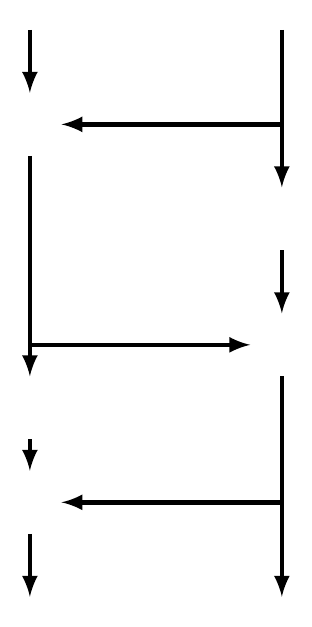
\begin{tikzpicture}[scale=0.8,ultra thick,>=latex]
% Reference grid (temporary)
%\draw[help lines] (0,0) grid (16,16);

% Inputs A and B
\drawMixerInputs
\draw[->] (1,15) to (1,14);
\draw[->] (5,15) to (5,12.5);

% Left adder 
\drawAdder{0.5}{14}
\draw[->] (5,13.5) to (1.5,13.5);

% Rotation
\drawRot{5}{12}

% Rotation
\drawRot{1}{9}
\draw[->] (1,13) to (1,9.5);

% Right adder
\drawAdder{4.5}{10.5}
\draw[->] (5,11.5) to (5,10.5);
\draw[->] (1,10) to (4.5,10);

% XOR
\drawXOR{1}{7.5}
\draw[->] (5,7.5) to (1.5,7.5);
\draw[->] (1,8.5) to (1,8);

% Outputs A' and B'
\draw[->] (1,7) to (1,6);
\draw[->] (5,9.5) to (5,6);
\drawMixerOutputs{10}
\end{tikzpicture}
\end{minipage}%
%
%
\begin{minipage}{.5\textwidth}
\vspace{1cm}
\centering
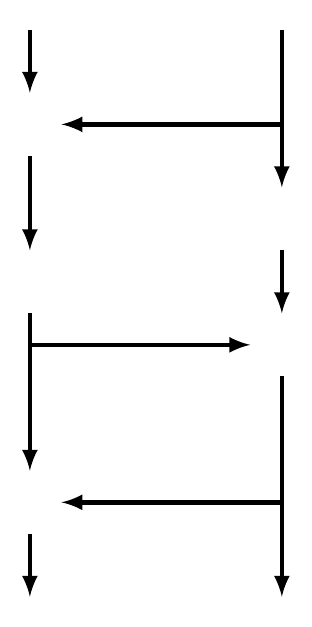
\begin{tikzpicture}[scale=0.8,ultra thick,>=latex]
% Reference grid (temporary)
%\draw[help lines] (0,0) grid (16,16);

% Inputs A and B
\drawMixerInputs
\draw[->] (1,15) to (1,14);
\draw[->] (5,15) to (5,12.5);

% Left adder 
\drawAdder{0.5}{14}
\draw[->] (5,13.5) to (1.5,13.5);

% Rotation
\drawRot{5}{12}

% Rotation
\drawRot{1}{11}
\draw[->] (1,13) to (1,11.5);

% Right adder
\drawAdder{4.5}{10.5}
\draw[->] (5,11.5) to (5,10.5);
\draw[->] (1,10) to (4.5,10);

% XOR
\drawXOR{1}{7.5}
\draw[->] (5,7.5) to (1.5,7.5);
\draw[->] (1,10.5) to (1,8);

% Outputs A' and B'
\draw[->] (1,7) to (1,6);
\draw[->] (5,9.5) to (5,6);
\drawMixerOutputs{10}
\end{tikzpicture}
\end{minipage}
%\caption{Custom candidate mixers with no initial rotation}
\caption{Custom candidate mixers}
\end{figure}

%%%%%%%%%%%%%%%%%%%%%%%%%%%%%%%%%%%%%%%

\begin{comment}
\begin{figure}[p]
\centering
\begin{minipage}{.5\textwidth}
\centering
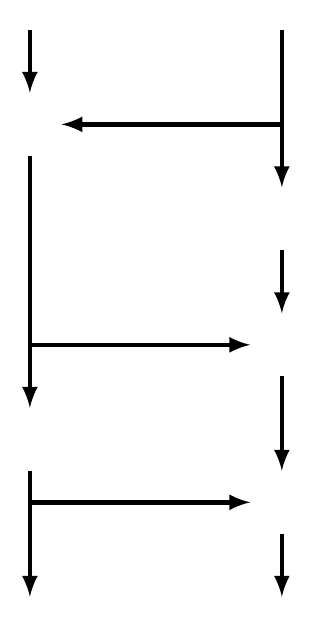
\begin{tikzpicture}[scale=0.8,ultra thick,>=latex]
% Reference grid (temporary)
%\draw[help lines] (0,0) grid (16,16);

% Inputs A and B
\drawMixerInputs
\draw[->] (1,15) to (1,14);
\draw[->] (5,15) to (5,12.5);

% Left adder 
\drawAdder{0.5}{14}
\draw[->] (5,13.5) to (1.5,13.5);

% Rotation
\drawRot{5}{12}

% Right adder
\drawAdder{4.5}{10.5}
\draw[->] (5,11.5) to (5,10.5);
\draw[->] (1,10) to (4.5,10);

% Rotation
\drawRot{1}{8.5}
\draw[->] (1,13) to (1,9);

% XOR
\drawXOR{5}{7.5}
\draw[->] (1,7.5) to (4.5,7.5);
\draw[->] (5,9.5) to (5,8);

% Outputs A' and B'
\draw[->] (1,8) to (1,6);
\draw[->] (5,7) to (5,6);
\drawMixerOutputs{10}
\end{tikzpicture}
\end{minipage}%
%
%
\begin{minipage}{.5\textwidth}
\centering
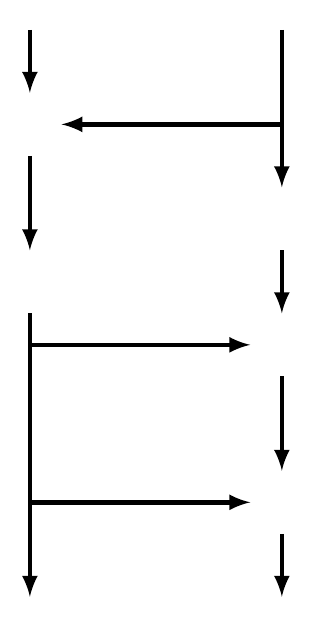
\begin{tikzpicture}[scale=0.8,ultra thick,>=latex]
% Reference grid (temporary)
%\draw[help lines] (0,0) grid (16,16);

% Inputs A and B
\drawMixerInputs
\draw[->] (1,15) to (1,14);
\draw[->] (5,15) to (5,12.5);

% Left adder 
\drawAdder{0.5}{14}
\draw[->] (5,13.5) to (1.5,13.5);

% Rotation
\drawRot{5}{12}

% Rotation
\drawRot{1}{11}
\draw[->] (1,13) to (1,11.5);

% Right adder
\drawAdder{4.5}{10.5}
\draw[->] (5,11.5) to (5,10.5);
\draw[->] (1,10) to (4.5,10);

% XOR
\drawXOR{5}{7.5}
\draw[->] (1,7.5) to (4.5,7.5);
\draw[->] (5,9.5) to (5,8);

% Outputs A' and B'
\draw[->] (1,10.5) to (1,6);
\draw[->] (5,7) to (5,6);
\drawMixerOutputs{10}
\end{tikzpicture}
\end{minipage}
%
%
\begin{minipage}{.5\textwidth}
\vspace{1cm}
\centering
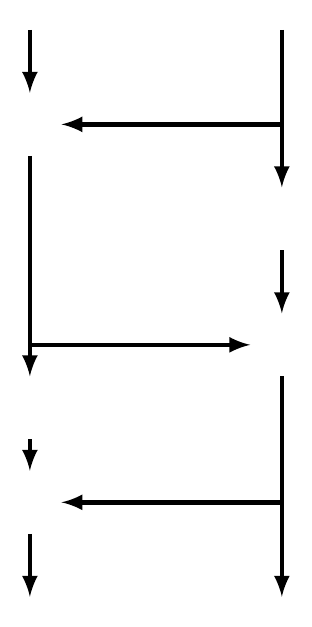
\begin{tikzpicture}[scale=0.8,ultra thick,>=latex]
% Reference grid (temporary)
%\draw[help lines] (0,0) grid (16,16);

% Inputs A and B
\drawMixerInputs
\draw[->] (1,15) to (1,14);
\draw[->] (5,15) to (5,12.5);

% Left adder 
\drawAdder{0.5}{14}
\draw[->] (5,13.5) to (1.5,13.5);

% Rotation
\drawRot{5}{12}

% Rotation
\drawRot{1}{9}
\draw[->] (1,13) to (1,9.5);

% Right adder
\drawAdder{4.5}{10.5}
\draw[->] (5,11.5) to (5,10.5);
\draw[->] (1,10) to (4.5,10);

% XOR
\drawXOR{1}{7.5}
\draw[->] (5,7.5) to (1.5,7.5);
\draw[->] (1,8.5) to (1,8);

% Outputs A' and B'
\draw[->] (1,7) to (1,6);
\draw[->] (5,9.5) to (5,6);
\drawMixerOutputs{10}
\end{tikzpicture}
\end{minipage}%
%
%
\begin{minipage}{.5\textwidth}
\vspace{1cm}
\centering
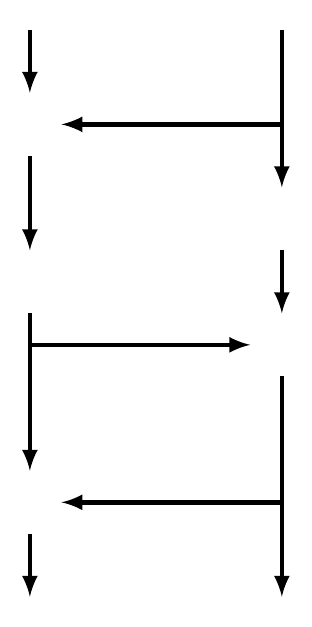
\begin{tikzpicture}[scale=0.8,ultra thick,>=latex]
% Reference grid (temporary)
%\draw[help lines] (0,0) grid (16,16);

% Inputs A and B
\drawMixerInputs
\draw[->] (1,15) to (1,14);
\draw[->] (5,15) to (5,12.5);

% Left adder 
\drawAdder{0.5}{14}
\draw[->] (5,13.5) to (1.5,13.5);

% Rotation
\drawRot{5}{12}

% Rotation
\drawRot{1}{11}
\draw[->] (1,13) to (1,11.5);

% Right adder
\drawAdder{4.5}{10.5}
\draw[->] (5,11.5) to (5,10.5);
\draw[->] (1,10) to (4.5,10);

% XOR
\drawXOR{1}{7.5}
\draw[->] (5,7.5) to (1.5,7.5);
\draw[->] (1,10.5) to (1,8);

% Outputs A' and B'
\draw[->] (1,7) to (1,6);
\draw[->] (5,9.5) to (5,6);
\drawMixerOutputs{10}
\end{tikzpicture}
\end{minipage}
\caption{Custom candiate mixers with initial rotation}
\end{figure}
\end{comment}
